% 2008 年江西卷理科第 20 题：正三棱锥 O-ABC，OA、OB、OC 两两垂直且长为 2；
%   E、F 为 AB、AC 中点，H 为 EF 中点；过 EF 的平面与 OA、OB、OC 的延长线交于 A1、B1、C1。
% 来源 PDF：gaokaomath-src/普通高考/2008/2008江西文.pdf
% SHA-256：8d079d71fadf20911ed2fd71acfe9562b94eb962cfe5228fe7a376f3b599b239
% 原页：2008江西理.pdf 第 2 页（A3 三栏）第 1 栏，书页码 460。
% 绘制依据：按原页斜投影：O 在上，A 在左、B 在下、C 在右；A1 在 OA 延长线上、C1 在 OC 延长线上、
%   B1 在 OB 延长线上；截面三角形 A1B1C1 为实线，EF 与 H 在内部（虚线）。
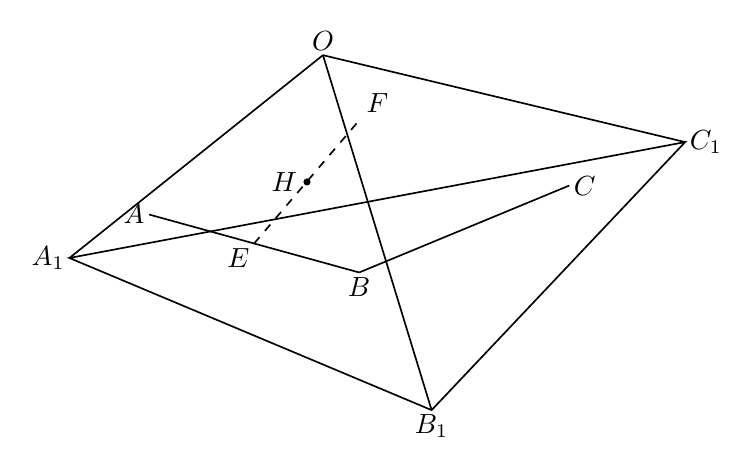
\begin{tikzpicture}[scale=0.92, semithick, every node/.style={inner sep=1.4pt}]
  \coordinate (O) at (2.60,4.30);
  \coordinate (A) at (0.20,2.10);
  \coordinate (B) at (3.10,1.30);
  \coordinate (C) at (6.00,2.50);
  \coordinate (A1) at (-0.90,1.50);
  \coordinate (B1) at (4.10,-0.60);
  \coordinate (C1) at (7.60,3.10);
  \coordinate (E) at (1.65,1.70);
  \coordinate (F) at (3.10,3.40);
  \coordinate (H) at (2.38,2.55);

  % 侧棱（延长后到 A1、B1、C1）
  \draw (O) -- (A1);
  \draw (O) -- (C1);
  \draw (O) -- (B1);

  % 截面三角形
  \draw (A1) -- (B1) -- (C1) -- cycle;

  % 底边
  \draw (A) -- (B);
  \draw (B) -- (C);

  % EF 与 H
  \draw[dashed] (E) -- (F);
  \fill (H) circle (1.4pt);

  \node[above] at (O) {$O$};
  \node[left] at (A) {$A$};
  \node[below] at (B) {$B$};
  \node[right] at (C) {$C$};
  \node[left] at (A1) {$A_1$};
  \node[below] at (B1) {$B_1$};
  \node[right] at (C1) {$C_1$};
  \node[below left] at (E) {$E$};
  \node[above right=1pt] at (F) {$F$};
  \node[left=2pt] at (H) {$H$};
\end{tikzpicture}
